\documentclass{IEEEtran}

\usepackage{amsmath}
\usepackage{listings}
\lstset{
    basicstyle=\small\ttfamily,
    breaklines=true
}
\usepackage{graphicx}
\graphicspath{ {./images/} }

\title{Readings about DP and Recursion}
\author{Diego Linares - kiwiAipom}

\begin{document}
    \maketitle

    \section{Everything about Dynamic Programming}

    \section{Some general approach for solving recursive problems}
        \textbf{Step One:} Think about any input for which you know what your function should return.\\
        Now suppose you have a task, related to a similar one. Keep calling that function to solve it: \textit{I'll solve the problem if you give me this subproblem first}. Which is done by a call to the same function.\\
        \textbf{Example:} With factorial, you only know that $0!=1$ and $n!=n(n-1)!$. So the function that gives me factorial of $n$ just needs the results of one that returns $(n-1)!$. This will keep going as long as we don't know whaat value to return.
        \begin{lstlisting}
factorial(n):
    if n = 0:
        return 1 // I know this, so I don't want my function to go any further
    else:
        return n*factorial(n-1) // just reuse the function
        \end{lstlisting}
        \textbf{Step Two:} They can do the same as loops, a simple \texttt{for} can be implemented as:
        \begin{lstlisting}
for(i, n):
    if i = n:
        return // Terminates
    // Do whatever needed
    for(i+1, n) // Next iteration
        \end{lstlisting}
        And for backwards:
        \begin{lstlisting}
rof(i, n):
    if i = n:
        return // Terminates
    rof(i+1, n) // Next iteration    
    // Do whatever needed
        \end{lstlisting}
        Since the function calls itself again until reaching a limit value and then starts returning.\\
        \textbf{Example:} To print numbers backwards you may do this:
        \begin{lstlisting}
function(i, n):
    if i <= n:
        function(i+1, n)
        print(i)
        \end{lstlisting}
        Which for numbers from 1 to 5 would work like:\\
        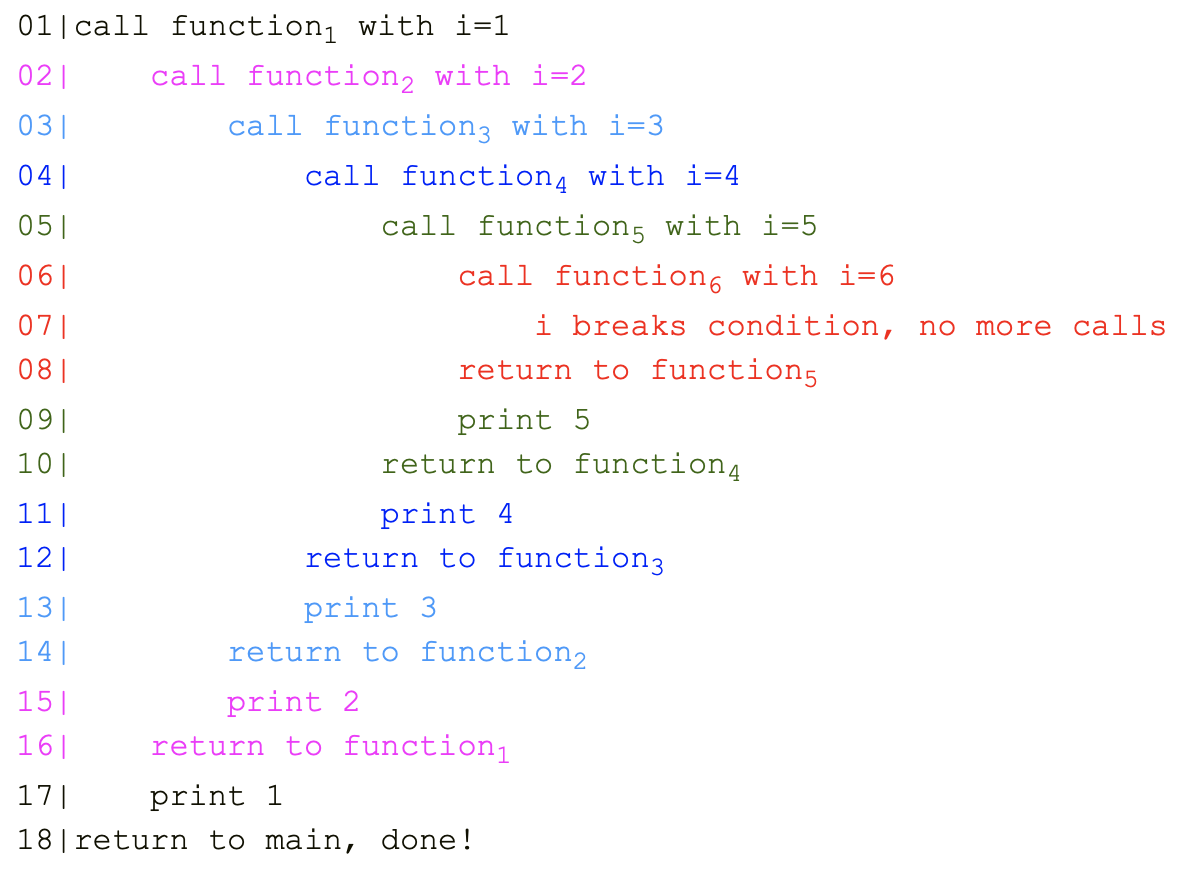
\includegraphics[width=0.4\textwidth]{rofExecution.png}\\
        \textbf{Step Three:} There's a stack call which looks like this:\\
        \begin{center}
            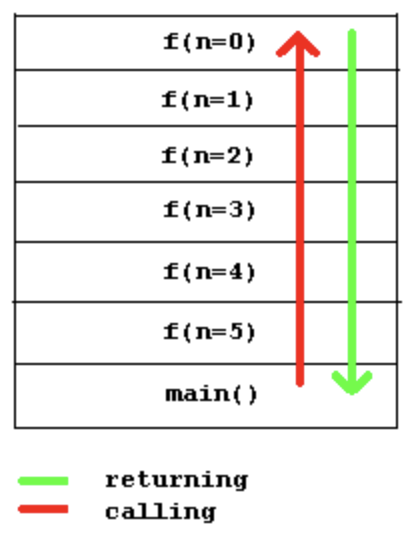
\includegraphics[width=0.15\textwidth]{stackCalls.png}
        \end{center}
        The memory of $f(3)$ for example, won't be freed until $f(2)$ is done. Serves the purpose of using an array, since the functions store variables and values.\\
        \textbf{Step Four:} Be careful, in CP they are generally avoided since most can be done iteratively, andd they may exceed time and memory. Since every function is alloted a space at the moment it is called, might run into RTE. Use only $O(\lg{n})$ and small $O(n)$ recursions. \\
        \textbf{Step Five:} When there are overlapping branches in the recursion tree we store computed values (DP).
    \section{Dynamic programming 2}
        \subsection{Longest Common Subsequence}
            2 strings $S,T$, find the LCS between them. Can be done in $O(S*T)$
            \begin{lstlisting}
int LCS(int n, int m) 
{
    if (n == 0 or m == 0) return 0;
    if (vis[n][m]) return memo[n][m];
    int &ans = memo[n][m] = max(LCS(n-1, m), LCS(n, m-1));
    if (S[n-1] == T[m-1]) ans = max(ans, 1 + LCS(n-1, m-1));
    vis[n][m] = 1;
    return ans;
}
            \end{lstlisting}
            It's trivial that if either of the strings is empty, there's no LCS.\\
            Next case is that $S[n-1],T[m-1]$ don't match any characters in the other string. If these two match though, we might have a new \texttt{ans}.\\
            The iterative alternative to this problem is:
            \begin{lstlisting}
for (int i = 0; i <= n; ++i) dp[i][0] = 0;
for (int i = 1; i <= m; ++i) dp[0][i] = 0;
for (int i = 1; i <= n; ++i) 
{
    for (int j = 1; j <= m; ++j) 
    {
		if (S[i-1] == T[j-1]) dp[i][j] = 1 + dp[i-1][j-1];
		else dp[i][j] = max(dp[i][j-1], dp[i-1][j]);
	}
}
            \end{lstlisting}
            Check that to obtain $(i,j)$ we need to preprocess $(i-1,j)$, $(i,j-1)$ and $(i-1,j-1)$
        \subsection{Kadane's Algorithm}
            $O(n)$ for maximum continuous subarray. 
            \begin{lstlisting}
int kadane(int pos) 
{
	if (pos == n) return 0;
	if (vis[pos]) return memo[pos];
	vis[pos] = 1;
  	return memo[pos] = a[pos] + max(0, kadane(pos+1));
}
            \end{lstlisting}    
            This finds the max sum starting in that position until the end of the array.\\
            If all were positive, I take all of them. I go checking and if the value adds to the sum, I memo the new value for that pos, otherwise, the memo for that pos is the same as the previous.\\
            We run this code for all pos, and obtain the maximum.\\
            Iteratively can be done as:
            \begin{lstlisting}
dp[0] = 0;
for (int i = 1; i <= n; ++i)
	dp[i] = a[i] + max(0, dp[i-1]);
            \end{lstlisting}
            It is also useful to \textbf{Check the Wikipedia implementation of it.}
            \begin{lstlisting}
def max_subarray(numbers):
    best_sum = 0  # or: float('-inf')
    current_sum = 0
    for x in numbers:
        current_sum = max(0, current_sum + x)
        best_sum = max(best_sum, current_sum)
    return best_sum
            \end{lstlisting}
        \subsection{Levenshtein's Distance}
            Two strings $S,T$, minimum amount of changes (elimination, change value, or adding) to make $S == T$. Can be solved recursively:
            \begin{lstlisting}
int editDistance(int n, int m) 
{ 
	if (n == 0 or m == 0) return n+m;
	if (vis[n][m]) return memo[n][m];
	int &ans = memo[n][m] = 1e9; //infinity
	ans = min(ans, editDistance(n-1, m-1) + s[n-1] != t[m-1]); // Change if necessary
	ans = min(ans, editDistance(n-1, m) + 1); // Eliminate the char
	ans = min(ans, editDistance(n, m-1) + 1); // Add a char after the n character
	vis[n][m] = 1;
	return ans;
}
            \end{lstlisting}
            So if either string is empty, answer is the length of the other string (delete all its elements).\\
            If those strings have already been checked, return its memo. And otherwise, start at infinity:
            \begin{itemize}
                \item We first check the $editDistance$ of the strings $-1$ char, and then check if the last chars are different.
                \item Then we check if we can eliminate a char from $S$
                \item And finally if we can add a char to $S$
            \end{itemize}
            The iterative implementation is:
            \begin{lstlisting}
dp[0][0] = 0;
for (int i = 1; i <= n; ++i) dp[i][0] = i;
for (int i = 1; i <= m; ++i) dp[0][i] = i;
for (int i = 1; i <= n; ++i) {
	for (int j = 1; j <= m; ++j) {
		dp[i][j] = min(
			dp[i-1, j-1] + s[i-1] != t[j-1],
			min(dp[i-1][j], dp[i][j-1]) + 1
		);
	}
}
            \end{lstlisting}
        \subsection{Rod cutting}
            Rod of lenght $n$, size $p_i$ and cost $r_i$ to cut each of the pieces. It's easy to see with an example:
            \begin{lstlisting}
length   | 1   2   3   4   5   6   7   8  
--------------------------------------------
price    | 3   5   8   9  10  17  17  20
            \end{lstlisting}
            In which case we can máximize the value (24 with 8 cuts of 1 lenght, or minimize it with 1 cut of lenght 8). The implementation for this first case is the following:
            \begin{lstlisting}
int rodCutting(int n) 
{
	if (n == 0) return 0;
	if (vis[n]) return memo[n];
	int &ans = memo[n] = INT_MAX;
    for (int i = 0; i < m; ++i) 
    {
		if (n >= p[i])
			ans = min(ans, r[i] + rodCutting(n-p[i]));
	}
	vis[n] = 1;
	return ans;
}
            \end{lstlisting}
            This is an implementation of a program in which $n$ is the length of the rod, but $m$ is the amount of ways you can cut it. $m \neq n$ is a possibility.
            So as always, the base is that if there's no rod, the price is 0, and if we already have the value, we return it.\\
            Then we start with the value on infinity. If $n$ is bigger than the size we are currently checking. We decided between the minimum of our current answer or, \textbf{the price of cutting the rod, plus the price of cutting a rod of minus that size}.\\
            Then we just add it to visited and we are done.\\
            Iteratively can be done as:
            \begin{lstlisting}
dp[0] = 0;
for (int i = 1; i <= n; ++i) dp[i] = 1e9;
for (int i = 0; i < m; ++i)
{
	for (int j = p[i]; j <= n; ++j) 
		dp[j] = min(dp[j], dp[j-p[i]] + r[i]);
	
}
            \end{lstlisting}
            Which is fairly similar.\\
            It is important to note that the \texttt{dp} array could be separated into 2 arrays with the same results. In its current state it has the states of the previous calc and the new ones. So be careful.

        \subsection{Longest Incresing Subsequence}
            Array of integers, the recursive implementation is the following.
            \begin{lstlisting}
void LIS(int pos) 
{
	if (n == 0) return 0;
	if (vis[pos]) return memo[pos];
	int &ans = memo[pos] = 1;
    for (int i = pos+1; i < n; ++i) 
    {
		if (a[pos] < a[i])
			ans = max(ans, 1 + LIS(i));
	}
	vis[pos] = 1;
	return ans;
}
            \end{lstlisting} 
            This code finds the maximum subarray starting at a position. So we have to save the biggest result of that function so far with a for ($O(n^2)$ in the end).\\
            \textbf{New plan:} $dp[k]$ will be the smalles value of a growing subsequence with $k$ elements. At the start $dp[0]=-\infty$ and $dp[i]=\infty$ for all $i>1$.\\
            To add $A[k]$, we search for the biggest element in $dp[i]$ which satisfies $dp[i] < A[k]$, and then we make $dp[i+1]=A[k]$, it becomes the best ending for a sequence of $i+1$ elements.\\
            In fact, since $dp$ is a growing array, we can use binary search to find the actual value to replace.
            \begin{lstlisting}
for (int i = 1; i <= n; ++i) dp[i] = INF;
dp[0] = -INF;
for (int i = 1; i <= n; ++i) 
{
	int lo = 0, hi = n;
    while (lo < hi) 
    {
		int mid = lo + (hi - lo) / 2; // This is the binary search part
		if (a[i] >= dp[mid]) lo = mid+1;
		else hi = mid;
	}
	dp[lo+1] = a[i];
}
            \end{lstlisting}

    \section{Matrix}
        \subsection{Cutting to the Chase}
            It can be slow if not done properly.\\
            \textbf{Example:} Obtain $x^n$ if multiplying is $O(1)$. Then $x^n=x*x*\ldots = O(N)$. We can reduce it like: $x^n=x^2*x^2*...$, and now the constant is now half. If we do $x^{\sqrt{n}}*x^{\sqrt{n}}*...$ and now the constant is $O(\sqrt{N})$\\
            So let's go faster. For even numbers $x^n=x^{\frac{n}{2}}*x^{\frac{n}{2}}$ and for odds $x^n = x^{\frac{n}{2}}*x^{\frac{n}{2}}*x$.\\
            Since the terms keep repeating themselves, we only need to calculate $x^{\frac{n}{2}}$ once and so on. This creates $O(\lg{n})$ complexity.\\
            Since matrices are an \textbf{associative mathematical structure}, this applies to it too.
        \subsection{Don't get stuck with struct}
            Matrix multiplication goes as such:\\
            $$
                \begin{bmatrix}
                    a_1&a_2\\
                    a_3&a_4
                \end{bmatrix}*
                \begin{bmatrix}
                    b_1&b_2\\
                    b_3&b_4
                \end{bmatrix}=
                \begin{bmatrix}
                    a_1*b_1+a_2*b_3&a_1*b_2+a_2*b_4\\
                    a_3*b_1+a_4*b_3&a_3*b_2+a_4*b_4
                \end{bmatrix}
            $$
            Basically, each row times each column of the other matrix. Now we can define a struct like:
            \begin{lstlisting}
struct Matrix
{
    int m[N][N];
    matrix()
    {
        memset(m,0,sizeof(m));
    }
    matrix operator * (matrix b)
    {
        matrix c = matrix();
        for(int i = 0; i < n; i++)
            for(int j = 0; j < n; j++)
                for(int k = 0; k < n; k++)
                    c.m[i][j] = c.m[i][j] + m[i][k] * b.m[k][j]
        return c;
    }
    matrix modPow(matrix m, int n)
    {
        if(n == 0)
            return unit;
        matrix half = modPow(m,n/2);
        matrix out = half * half;
        if(n % 2)
            out *= m;
        return out;
    }
}
            \end{lstlisting}
            The operator $*$ was defined so the matrix could be treated as a number. Unit refers to the unit matrix. 
        \subsection{N-th Fibonacci Term}
            Knowing how Fibonacci works, we can put it in the form of a matrix. Knowing that each term \textbf{is dependent on the previous two} we need a 2 row matrix. From the pair $(F_{n-2},F{n_1})$ we compute $(F_{n-1},F{n})$, like so:
            $$F_n=F_{n-1}*1+F_{n-2}*1$$
            $$F_{n-1}=F_{n-1}*1+F_{n-2}*0$$
            In the form of a matrix:
            $$
                \begin{bmatrix}
                    F_{n-2}&F_{n-1}\\
                    0&0
                \end{bmatrix}*
                \begin{bmatrix}
                    0&1\\
                    1&1
                \end{bmatrix}=
                \begin{bmatrix}
                    F_{n-1}&F_{n}\\
                    0&0
                \end{bmatrix}
            $$
            We can go one step back to see the pattern:
            $$
                \begin{bmatrix}
                    F_{n-3}&F_{n-2}\\
                    0&0
                \end{bmatrix}*
                \begin{bmatrix}
                    0&1\\
                    1&1
                \end{bmatrix}^2=
                \begin{bmatrix}
                    F_{n-2}&F_{n-1}\\
                    0&0
                \end{bmatrix}
            $$
            Finally
            $$
                \begin{bmatrix}
                    F_{1}&F_{2}\\
                    0&0
                \end{bmatrix}*
                \begin{bmatrix}
                    0&1\\
                    1&1
                \end{bmatrix}^{n-2}=
                \begin{bmatrix}
                    F_{n-1}&F_{n}\\
                    0&0
                \end{bmatrix}
            $$
            And we already know the power of a matrix is logarithmic.
        \subsection{Bits and Pieces}
            How many arrays of length $n$ with maximum $k$ consecutive 0 bits are.\\
            Supposing we can use DP for the problem. $D_{n.k}$ is the number of arrays of length $n$ which \textbf{end} in $k$ 0s.\\
            Considering a string can only be added a 0 or a 1. From $(n,k)$ we can go to $(n+1,k+1)$ (if we add 0) and $(n+1,0)$ (we add 1).\\
            So $D_{n,0} = \sum_{i=0}^k D_{n-1,i}$ (all the strings of length n which do not end in 0). And $D_{n,k}=D_{n-1,k-1}.$ So in recursive form:
            $$D_{n,0} = \sum_{i=0}^k D_{n-1,i}$$
            $$D_{n,1} = D_{n-1,0}$$
            $$D_{n,2} = D_{n-1,2}$$
            $$\cdots$$
            $$D_{n,k} = D_{n-1,k-1}$$
            And this can be explained through a matrix.
            $$
            \begin{bmatrix}
                D_{n-1,0}&D_{n-1,1}&\cdots&D_{n-1,k}\\
                0&0&\cdots&0\\
                \cdots&\cdots&&\cdots\\
                0&0&\cdots&0\\
                0&0&\cdots&0
            \end{bmatrix}*
            \begin{bmatrix}
                1&1&\cdots&0\\
                1&0&\cdots&0\\
                \cdots&\cdots&&\cdots\\
                1&0&\cdots&1\\
                1&0&\cdots&0
            \end{bmatrix}
            $$
            Yielding the result:
            $$
            \begin{bmatrix}
                D_{n,0}&D_{n,1}&\cdots&D_{n,k}\\
                0&0&\cdots&0\\
                \cdots&\cdots&&\cdots\\
                0&0&\cdots&0\\
                0&0&\cdots&0
            \end{bmatrix}
            $$
            The complexity is reduced from $O(n*k)$ to $O(\lg{n}*k^3)$, where $k^3$ is the complexity of multiplying the matrices. 
        \subsection{How big can it get?}
            This is a solution to the problem \textit{Chimney} from TopCoder. \textbf{Worth checking out}.
            \begin{lstlisting}
Layer 1      Layer 2
+-----+--+   +--+-----+
|  1  |  |   |  |  B  |
+--+--|2 |   | A+--+--+
|  |  |  |   |  |  |  |
| 4+--+--+   +--+--+C |
|  |  3  |   |  D  |  |
+--+-----+   +-----+--+
            \end{lstlisting}
            We need to find out the different orders in which bricks can be placed for $n$ layers, only restriction is that the 2 bricks that support the brick above are set before it.\\
            We can show it as a matrix here:
            \begin{lstlisting}
+-----+--+  +-----+--+  +-----+--+  +-----+--+ 
|xxxxx|  |  |     |  |  |xxxxx|  |  |     |xx|  
+--+--|  |  +--+--|  |  +--+--|  |  +--+--|xx|    
|  |  |  |  |xx|  |  |  |  |  |  |  |xx|  |xx|    
|  +--+--+  |xx+--+--+  |  +--+--+  |xx+--+--+  
|  |     |  |xx|xxxxx|  |  |xxxxx|  |xx|xxxxx|  
+--+-----+  +--+-----+  +--+-----+  +--+-----+   
    1            2           3           4

+-----+--+  +-----+--+  +-----+--+  +-----+--+
|     |  |  |     |xx|  |     |xx|  |     |xx|
+--+--|  |  +--+--|xx|  +--+--|xx|  +--+--|oo| 
+--+--|  |  +--+--|xx|  +--+--|xx|  +--+--|oo|
|xx|  |  |  |xx|  |oo|  |xx|  |oo|  |xx|  |oo|
|xx+--+--+  |xx+--+oo+  |xx+--+oo+  |xx+--+oo+
|=====xxx|  |xx|xxxoo|  |===== oo|  |===@@@@@|  
+--+-----+  +--+-----+  +--+-----+  +--+-----+ 
    5            6           7           8
            \end{lstlisting}
            Where $x$ are the bricks in $n$ layer, $o$ and $=$ in the $n+1$ and $@$ in the $n+2$. After we place 2 bricks next to the other we can put a brick in the layer above.\\
            Can be solved with matrix multiplication, $9*9$ matrix and multiplying it logarithmically. The base matrix being:
            \begin{lstlisting}
int mat[9][9] =  // constructing matrix column by column
    {{0,0,0,0,1,0,0,0,0},
    {4,0,0,0,0,0,1,0,0},
    {0,2,0,0,0,0,0,1,0},
    {0,1,0,0,0,0,0,0,0},
    {0,0,2,2,0,0,0,0,0},
    {0,0,1,0,0,0,0,0,1},
    {0,0,0,0,2,2,0,0,0},
    {0,0,0,0,0,0,1,0,0},
    {0,0,0,0,0,0,0,1,0}};
            \end{lstlisting}
        \subsection{Summing Up}
            Useful tool but not reccommended outside of contests.

\begin{thebibliography}{}
    \bibitem{mmi}
        \textit{Attacking Recursions},
        I, Me and Myself.
        From: https://zobayer.blogspot.com/2009/12/cse-102-attacking-recursion.html
    \bibitem{mini}
        Miguel Mini,
        \textit{Dynamic Programming 2},
        miguelAlessandro's CompetitiveProgramming,
        From: https://github.com/miguelAlessandro/CompetitiveProgramming
    \bibitem{danalex}
        \textit{Matrix},
        DanAlex's blog,
        From: https://codeforces.com/blog/entry/21189


\end{thebibliography}

\end{document}